\documentclass[t,usenames,dvipsnames]{beamer} % [t] pomeni poravnavo na vrh slida

% \usepackage{etex} % vključi ta paket, če ti javi napako, da imaš naloženih preveč paketov.

% standardni paketi
\usepackage[slovene]{babel}
\usepackage[T1]{fontenc}
\usepackage[utf8]{inputenc}
% \usepackage{amssymb}
% \usepackage{amsmath}
%\usepackage{diagrams}

\useoutertheme{infolines}

\setbeamercovered{invisible} %default
% \setbeamercovered{transparent}
%\setbeamercovered{dynamic}


% podatki
\title{Demo}
% \author{Boštjan Gec}

% \usetheme{Singapore}
% \usetheme{Luebeck}
\usetheme{Frankfurt}
% \usecolortheme{crane}
% \usecolortheme{red}

% DIY  % % % % % % % % % % % % % % % % % % % % % 
%colors:
%\documentclass[usenames,dvipsnames]{beamer}
\usepackage{color}
%\usepackage[usenames,dvipsnames,svgnames,table]{xcolor}
% \setbeamercolor{structure}{fg=Bittersweet} 

% vscode colors (in rgb):
% green: 22,130,93
% blue: 0,122,204
% windowsLightBlue 210,228,239
% vscodegray = 44,44,44
\definecolor{greenvscode}{RGB}{22,130,93}
% \definecolor{bluevscode}{RGB}{0,122,204}
% \definecolor{vscodeGray}{RGB}{44,44,44}
% \definecolor{vscodeLightBlue}{RGB}{210,228,239}

\setbeamercolor{structure}{fg=greenvscode}
% \setbeamercolor{structure}{fg=bluevscode}
% \setbeamercolor{structure}{fg=vscodeGray}
% \setbeamercolor{structure}{fg=vscodeLightBlue}
% \setbeamercolor{structure}{bg=black}

% \setbeamercolor{background canvas}{bg=black}

% \usepackage{layout}

\newlength{\fullHDwidth}
\newlength{\fullHDheight}
\setlength{\fullHDwidth}{1920pt}
\setlength{\fullHDheight}{1080pt}
\newlength{\mywidth}
\newlength{\myheight}
\setlength{\mywidth}{0.25\fullHDwidth}
\setlength{\myheight}{0.25\fullHDheight}

% \setlength{\textwidth}{6.5in}
% \setlength{\hoffset}{-72.27pt}
% \setlength{\hoffset}{\mywidth}
% \setlength{\hoffset}{-27pt}
% \setlength{\hoffset}{-0.96cm}
% \addtolength{\hoffset}{-0.5cm}
% \addtolength{\hoffset}{-0.5cm}
% \addtolength{\topmargin}{2cm}
\addtolength{\headsep}{0.65cm}
% \addtolength{\headsep}{-0.6cm}
% \addtolength{\topmargin}{-2cm}
% \addtolength{\headheight}{-2cm}
% \addtolength{\headheight}{0cm}

% \setlength{}{-0.96cm}
% \addtolength{\oddsidemargin}{-0.4cm}
% \setlength{\marginparsep}{0pt}
% \setlength{\marginparwidth}{0pt}
% \addtolength{\paperwidth}{3cm}
% \setlength{\paperwidth}{1280pt}
% \setlength{\paperheight}{720pt}
% \setlength{\paperwidth}{1920pt}
% \setlength{\paperheight}{1080pt}
\setlength{\paperwidth}{\mywidth}
\setlength{\paperheight}{\myheight}
% \addtolength{\marginparsep}{-0.5cm}
% \addtolength{\marginparwidth}{-2cm}
\addtolength{\footskip}{1.2cm}
% \setlength{\textheight}{\myheight minus \footskip}
% \setlength{\textheight}{0.1\myheight}


\usepackage{geometry}

% \usetheme{CambridgeUS}
% \setbeamertemplate{page number in head/foot}[appendixframenumber]

\usepackage{showframe}


% \useoutertheme{miniframes}
% \useoutertheme{shadow}
% \useoutertheme{sidebar}
% \useoutertheme{smoothbars}
% \useoutertheme{smoothtree}
% \useoutertheme{split}
% \useoutertheme{tree}

\begin{document}


\begin{frame}
  \maketitle
\end{frame}

% \begin{frame}[shrink]

\newgeometry{margin=-0.5cm}
\begin{frame}[plain]
	\begin{center}
	% \includegraphics[width=\paperwidth]{fullcode3.png}
\includegraphics[height=1.1\paperheight]
{fullcode3.png}
	\end{center}
\end{frame}
\restoregeometry

% \newgeometry{top=0cm, left=0cm}
\newgeometry{left=0cm}
	% dsadsadsadsadsadsadsadsadsa \the\footskip 
	% textheight: \the\textheight
\begin{frame}
	\begin{center}
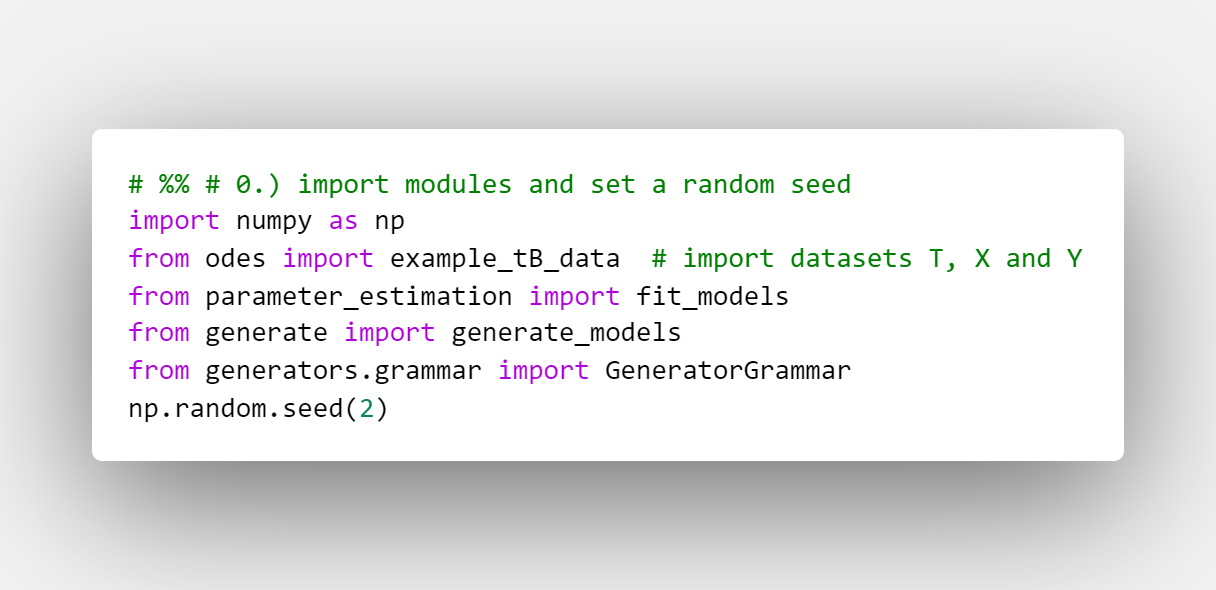
\includegraphics[width=\paperwidth]
{code-shots/0imports.png}				
	\end{center}
	% \insertframenumber/\inserttotalframenumber
\end{frame}

\begin{frame}
	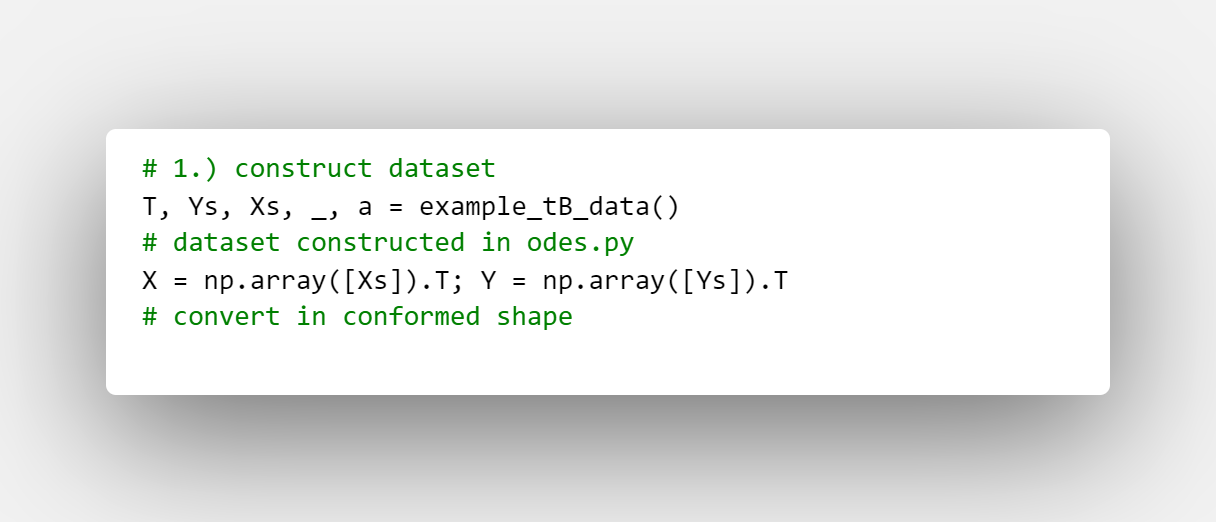
\includegraphics[width=\paperwidth]
{code-shots/1dataset-construction.png}
\end{frame}
\restoregeometry

\newgeometry{left=-1cm}
\begin{frame}
	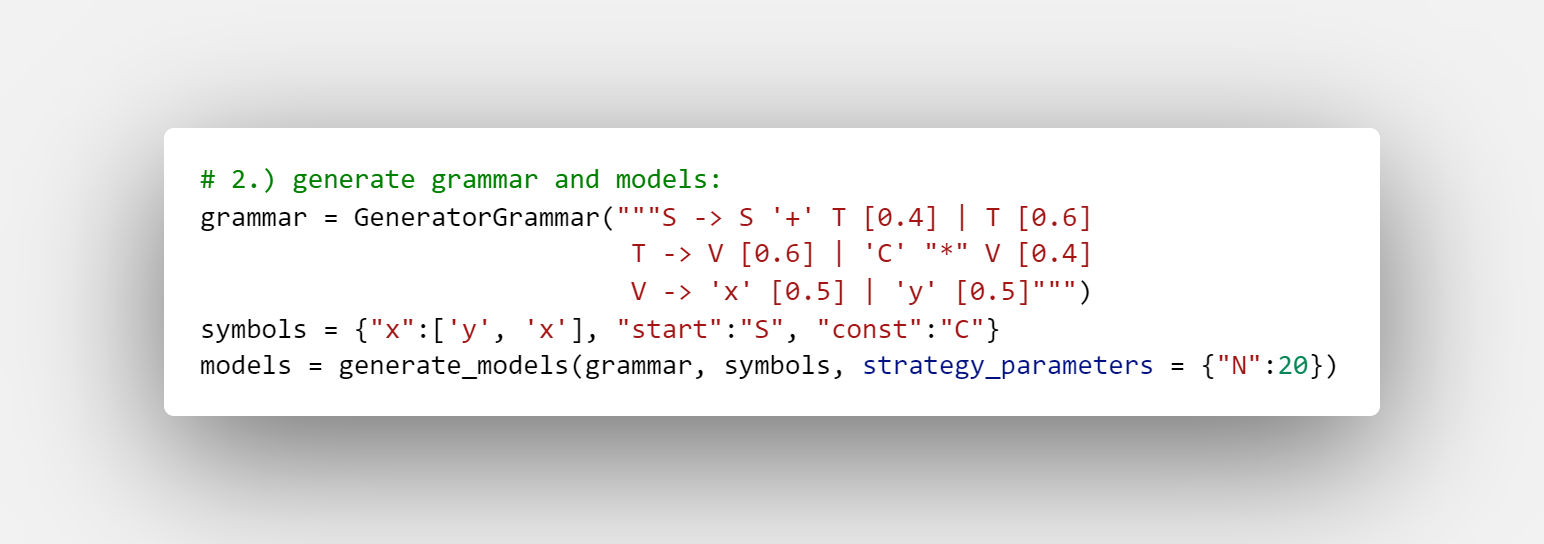
\includegraphics[width=1.15\paperwidth]
{code-shots/2grammar.png}
\end{frame}
\restoregeometry

\newgeometry{left=-1.5cm}
\begin{frame}
	\begin{center}
		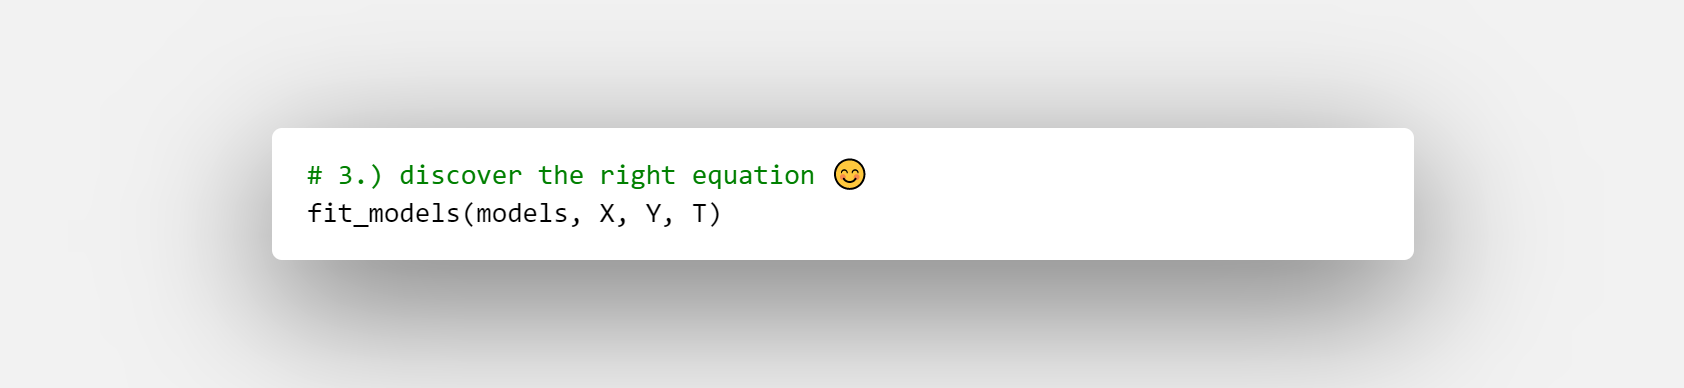
\includegraphics[width=1.2\paperwidth]
{code-shots/3eqDisco.png}	
	\end{center}
\end{frame}
\restoregeometry

\newgeometry{left=0cm}
\begin{frame}
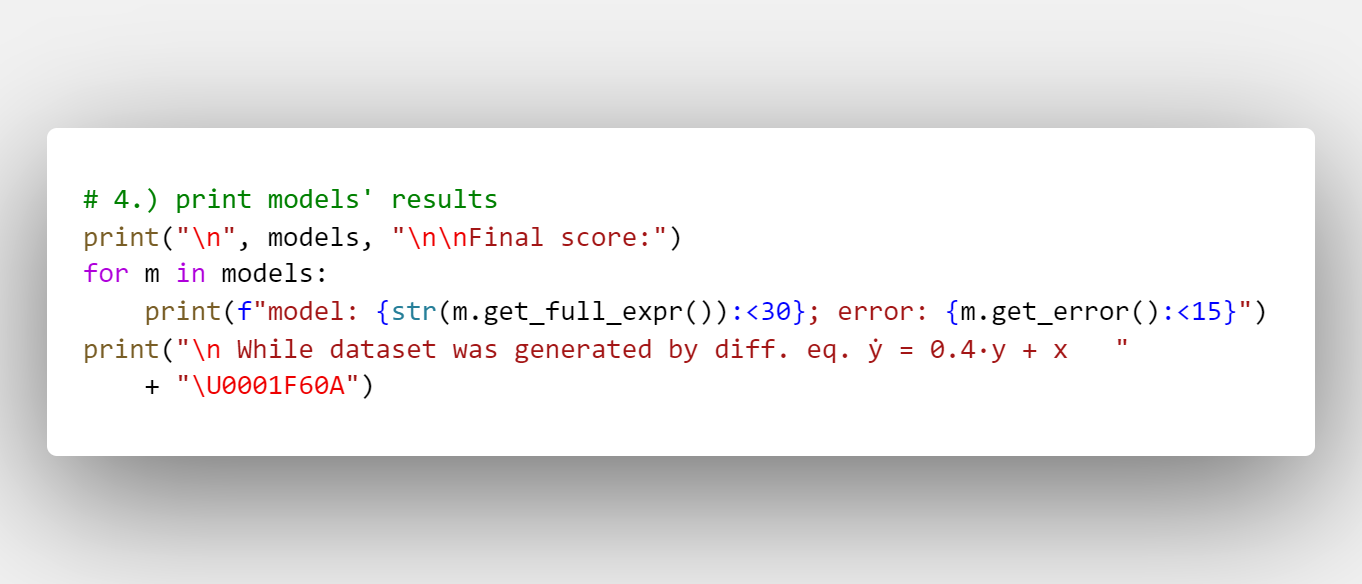
\includegraphics[width=1\paperwidth]
{code-shots/4print-models.png}
\end{frame}
\restoregeometry

\newgeometry{left=0cm, top=0.5cm}
% \newgeometry{left=0cm}
\begin{frame}[plain]

\includegraphics[height=1cm]
{code-shots/4_1runInTerminal2.png} \pause
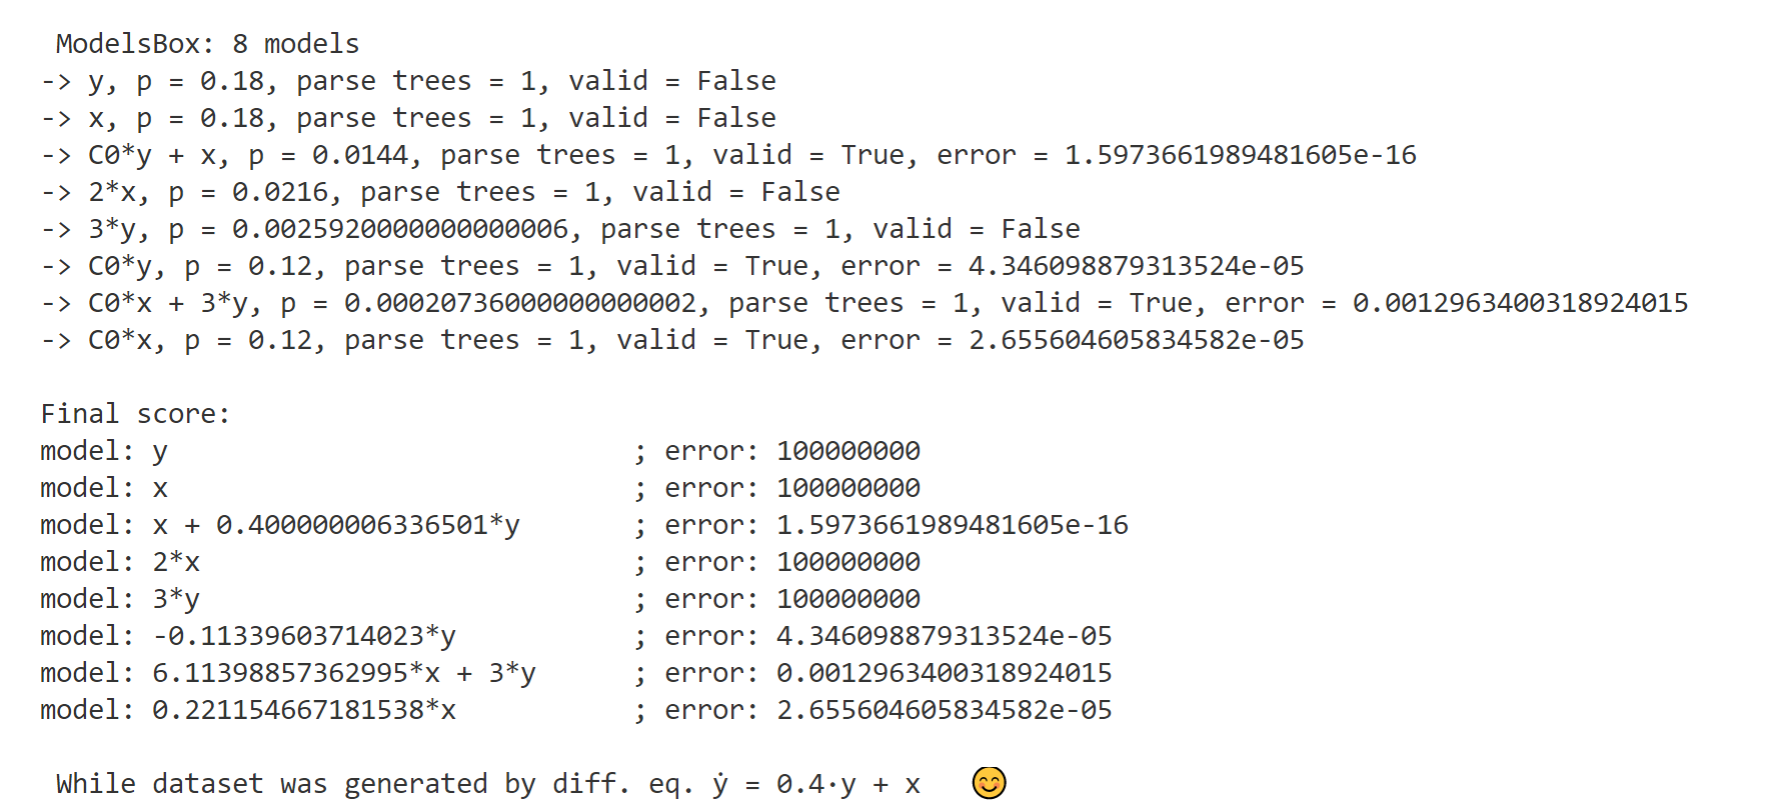
\includegraphics[width=\paperwidth]
{code-shots/4_2run-result-edd.png} 
\end{frame}
\restoregeometry

\newgeometry{left=-1cm}
\begin{frame}
	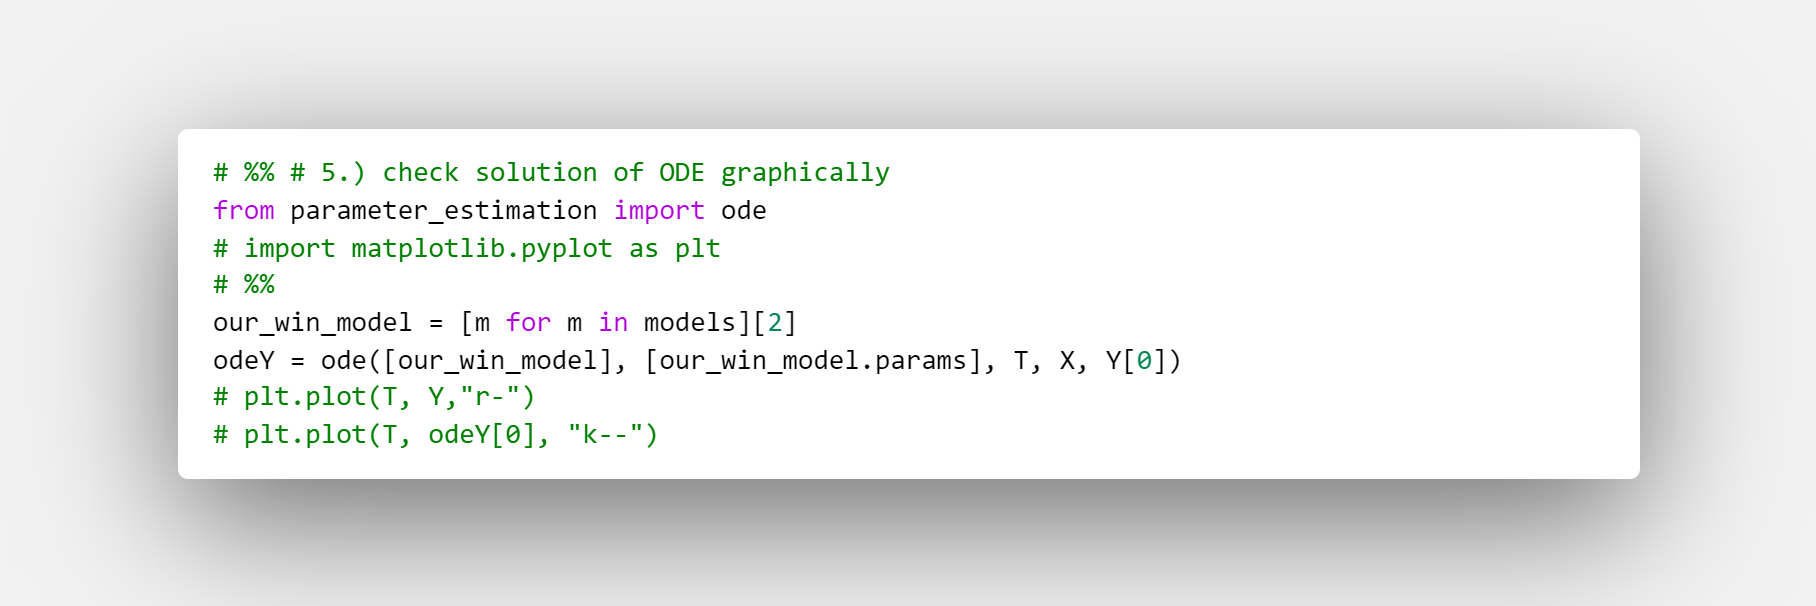
\includegraphics[width=1.1\paperwidth]
	{code-shots/5graphic-check.png}
\end{frame}
\restoregeometry

% \newgeometry{top=-0.1cm, left=0cm}
\newgeometry{left=1.5cm}
\begin{frame}
	% \begin{center}
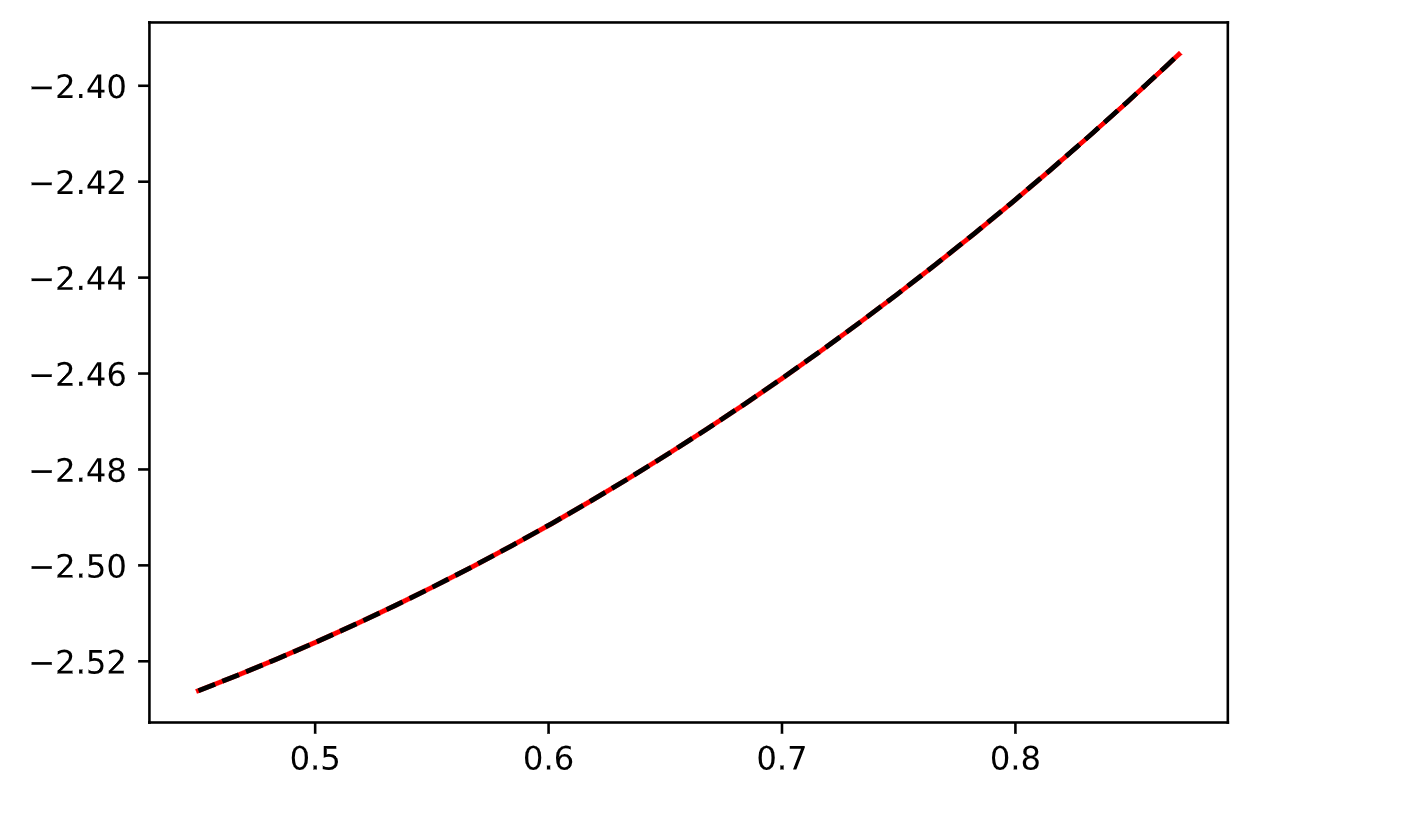
\includegraphics[height=0.85\paperheight]
{code-shots/5_1plotScr.png}
	% \end{center}
\end{frame}


\section{Uvod}

\begin{frame}
	% {Uvod}

	\begin{itemize}
		\item V programiranju so seznami in drevesa pomembne (in uporabne) podatkovne strukture.
		
		\item V modernih programskih jezikih (npr. jaz bom uporabljal Haskell) lahko skonstruiramo podatkovne tipe za sezname in drevesa.
		
		\item Te podatkovne tipe lahko karakteriziramo z za"cetnimi algebrami in tudi kon"cnimi koalgebrami.
		
		\item Ta karakterizacija nam daje metode in na"cine pri programiranju s seznami in drevesi.
	\end{itemize}
\end{frame}

\section{demo}

\begin{frame}
	% {Za"cetne algebre in kon"cne koalgebre}
	\begin{itemize}
		\item 	Za"cetna algebra in kon"cna koalgebra sta koncepta iz teorije kategorij.
		
		\item 
		
		\item V predstavitvi bom namesto splo"sne definicije predstavil njeno bolj zo"zeno verzijo na enem pomembnem primeru.
		
		\item Izbran primer: seznami v programiranju in njihov analog v matematiki: zaporedja.
		
		\item 
	\end{itemize}
\end{frame}

\section{todo}

\begin{frame}
	% {Seznami}
	Nekaj primerov seznamov:
	\begin{itemize}
		\item	 \text{[1, 2, 3, 4, 5]}
		\item	\text{[1, 3, 5]}
		\item	\text{[  \ ]}
	\end{itemize}
	
	... [Int]	\\
	Seznami razli"cnih tipov:
	\begin{itemize}
		\item	$[\frac{1}{2},\frac{2}{3},\frac{10}{7}]$ ... \text{[Fractional]}
		\item	\text{[0.01, pi, e, 2.04]}  ... \text{[Floating]}
		\item	\text{['p', 'i', 'e'] }      ... \text{[Char]}
		\item	\text{[ [0,1,2,3], [\ \  ], [3] ]}  ... \text{[[Int]]}
	\end{itemize}	
\end{frame}
\restoregeometry

\end{document}
